% ex: ts=2 sw=2 sts=2 et filetype=tex
% SPDX-License-Identifier: CC-BY-SA-4.0

\documentclass{article}

\usepackage[T1]{fontenc}
\usepackage[utf8]{inputenc}
%\usepackage[spanish]{babel}
\usepackage{pgfplots}

\begin{document}
  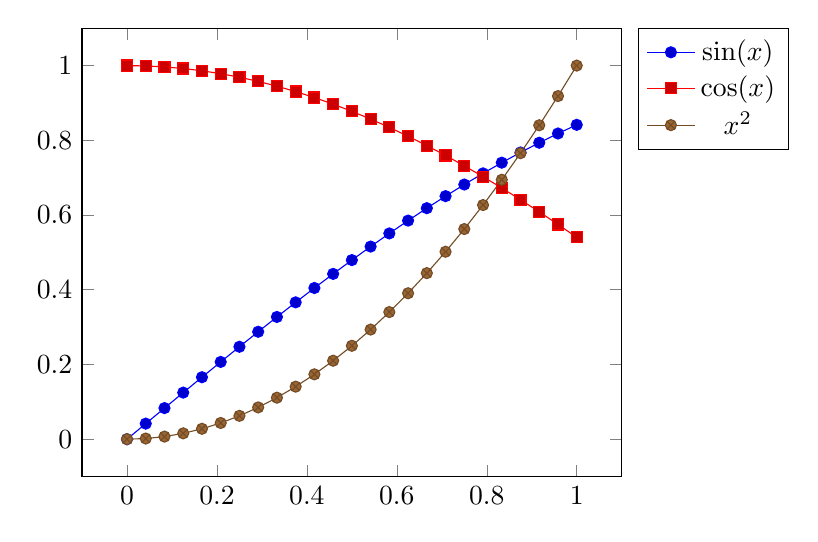
\begin{tikzpicture}
    \begin{axis}[domain=0:1,legend pos=outer north east]
    \addplot {sin(deg(x))}; 
    \addplot {cos(deg(x))}; 
    \addplot {x^2};
    \legend{$\sin(x)$,$\cos(x)$,$x^2$}
    \end{axis}
  \end{tikzpicture}

\begin{tikzpicture}[domain=0:4]
  \draw[dotted] (0,0) grid (3,2);
  \draw[->] (0,0) -- (1,0);
  
  %\draw[very thin,color=gray] (-0.1,-1.1) grid (3.9,3.9);
  %\draw[->] (-0.2,0) -- (4.2,0) node[right] x;
  %\draw[->] (0,-1.2) -- (0,4.2) node[above] {$f(x)$};
\end{tikzpicture}

\end{document}
